% Template:     Informe LaTeX
% Documento:    Archivo de ejemplo
% Versión:      7.0.0 (23/06/2020)
% Codificación: UTF-8
%
% Autor: Pablo Pizarro R.
%        Facultad de Ciencias Físicas y Matemáticas
%        Universidad de Chile
%        pablo@ppizarror.com
%
% Manual template: [https://latex.ppizarror.com/informe]
% Licencia MIT:    [https://opensource.org/licenses/MIT]

% ------------------------------------------------------------------------------
% NUEVA SECCIÓN
% ------------------------------------------------------------------------------
% Las secciones se inician con \section, si se quiere una sección sin número se
% pueden usar las funciones \sectionanum (sección sin número) o la función
% \sectionanumnoi para crear el mismo título sin numerar y sin aparecer en el índice

\newcommand{\explorelite}{\textit{explore\_lite}}
\newcommand{\movebase}{\textit{move\_base}}

\section{Pregunta 1}

\subsection{Parte a.-}

\begin{figure}
    \centering
    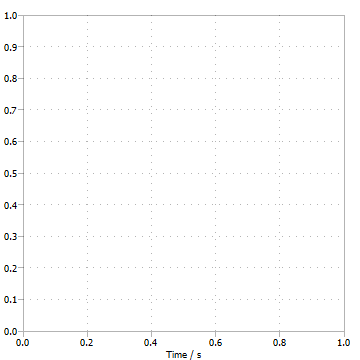
\includegraphics[width=0.5\linewidth]{Tarea 1/report/imanges/Viabc_dg1.png}
    \caption{Caption}
    \label{fig:enter-label}
\end{figure}

\subsection{Parte b.-}



\subsection{Parte c.-}



\subsection{Parte d.-}



\subsection{Parte e.-}



\section{Pregunta 2}

\subsection{Parte a.-}



\subsection{Parte b.-}



\subsection{Parte c.-}



\section{Pregunta 3}

\subsection{Parte a.-}



\subsection{Parte b.-}



\subsection{Parte c.-}



\subsection{Parte d.-}



\section{Extras}

\subsection{Parte a.-}



\subsection{Parte b.-}



